\section{The EM meta-rewrite}

\begin{definition}
The EM meta-rewrite is: If $b, c$ are terms such that $\displaystyle b \leftrightarrow c$  and $\displaystyle d \in \Upsilon \cup \left\{ 0 , 1 \right\}$ then 
$$\displaystyle (La.b) d \stackrel{EM}{\longleftrightarrow} (La.c) d$$
An emergent rewrite is any chain $a \longleftrightarrow b$ of rewrites, where $a, b$ are terms and the chain contains at least a EM meta-rewrite. 
\end{definition}



\begin{figure}[h]\centerline{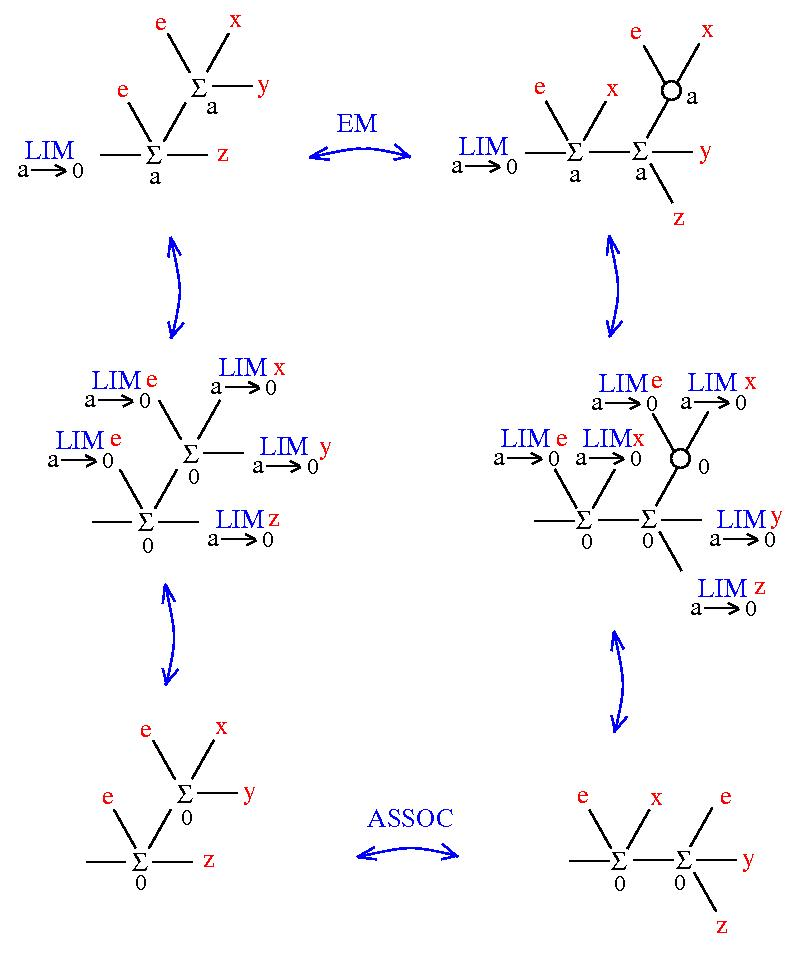
\includegraphics[width=120mm]{jpg/sumassoc-em.jpg}}  \caption{ The ASSOC rewrite is emergent. The EM meta-rewrite is applied for the rewrite from the Figure \ref{sumassoc}} \label{sumassoc-em-fig} \end{figure}

An example of an emergent rewrite is ASSOC, described in the Figure \ref{sumassoc-em-fig}. We use the Figure \ref{sumassoc} and we apply the EM meta-rewrite: for $e, x, y, z$ terms which don't contain the node variable $a$ 
$$ \displaystyle \left(La.\Sigma_{a}^{e}\left( \Sigma_{a}^{e}\left(x,y\right), z\right)\right) 0 \, \stackrel{EM}{\longleftrightarrow} \, \left(La.\Sigma_{a}^{e}\left( x, \Sigma_{a}^{a^{e} x} \left( y,z\right)\right)\right) 0 $$
The limterm from the left hand side reduces, via LIM rewrites, as described in the left column of the Figure \ref{sumassoc-em-fig}: 
$$ \displaystyle \left(La.\Sigma_{a}^{e}\left( \Sigma_{a}^{e}\left(x,y\right), z\right)\right) 0 \, \stackrel{LIM}{\longleftrightarrow} \, $$ 
$$ \Sigma_{0}^{(La.e)0}\left( \left( La.\Sigma_{a}^{e}\left(x,y\right)\right) 0, (La.z)0\right) \, \stackrel{LIM}{\longleftrightarrow} \, $$ 
$$\Sigma_{0}^{e}\left( \Sigma_{0}^{(La.e) 0}\left((La.x)0,(La.y)0\right), z\right) \, \stackrel{LIM}{\longleftrightarrow} \, \Sigma_{0}^{e}\left( \Sigma_{0}^{e}\left(x,y\right), z\right)$$
In all detail there were 7 LIM rewrites and the last expression is a term. The limterm from the right hand side reduces in a slightly longer way: 
$$ \displaystyle  \left(La.\Sigma_{a}^{e}\left( x, \Sigma{a}^{a^{e} x} \left( y,z\right)\right)\right) 0 \, \stackrel{LIM}{\longleftrightarrow} \, $$ 
$$\Sigma_{0}^{(La.e) 0}\left( (La.x)0, La.\left(\Sigma_{a}^{a^{e} x} \left( y,z\right)\right) 0\right) \, \stackrel{LIM}{\longleftrightarrow} \, $$ 
$$ \Sigma_{0}^{e}\left( x , \Sigma_{0}^{\left(La.a^{e} x\right) 0} \left( (La.y) 0, (La.z) 0\right)\right) \, \stackrel{LIM}{\longleftrightarrow} \, $$
$$ \Sigma_{0}^{e}\left( x , \Sigma_{0}^{0^{(La.e) 0} (La.x) 0} \left( y, z\right)\right) \, \stackrel{LIM}{\longleftrightarrow} \, $$
$$ \Sigma_{0}^{e}\left( x , \Sigma_{0}^{0^{e} x} \left( y, z\right)\right) \, = \, \Sigma_{0}^{e}\left( x , \Sigma_{0}^{e} \left( y, z\right)\right)   $$
In this case there were 9 LIM rewrites until we obtain a term, then we use the definition of the term $0$ at the end.

We obtain the emergent rewrite: 
$$\Sigma_{0}^{e}\left( \Sigma_{0}^{e}\left(x,y\right), z\right) \, \stackrel{ASSOC}{\longleftrightarrow} \, \Sigma_{0}^{e}\left( x , \Sigma_{0}^{e} \left( y, z\right)\right)   $$
which expresses, in abstract syntactic tree (AST) form, the fact that for any term $e$ the operation $\displaystyle \Sigma_{0}^{e}(\cdot, \cdot)$ is associative. Mind that the operation itself is emergent: for any $e, x, y$ terms which don't contain the node variable $a$ 
$$(\left(La. \Sigma_{a}^{e}(x,y)\right) 0  \, \stackrel{LIM}{\longleftrightarrow} \, \Sigma_{0}^{(La.e) 0} \left((La.x) 0 , (La.y) 0) \right)  \, \stackrel{LIM}{\longleftrightarrow} \, \Sigma_{0}^{e}(x,y)$$
Therefore, we are able to obtain emergent algebraic structures (operations) and properties of those (like associativity here) from the LIM rewrites of limterms, on one side, and from the use of the EM meta-rewrite with term rewrites, on the other side. 

